\documentclass{article}

\usepackage{lipsum}
\usepackage[letterpaper, margin=1.4in]{geometry}
\usepackage{float}

%
\usepackage{tikz}
%
\usetikzlibrary{calc}
%
\usepackage{graphicx}
\usepackage{setspace}

\graphicspath{ {c:/Users/User/Documents/thesis/Thesis/thesisimages/} }


\begin{document}

\begin{titlepage}

\begin{tikzpicture}[overlay,remember picture]
    \draw [line width=1pt,rounded corners=0pt,
        ]
        ($ (current page.north west) + (2cm,-2cm) $)
        rectangle
        ($ (current page.south east) + (-2cm,2cm) $);
\end{tikzpicture}

    \begin{center} 
	\Large
        \vspace*{1cm}
        
        \textbf{ Integrated Deep Learning and Bayesian Classification for Prioritization of Functional Genes in Next-Generation Sequencing Data }
        
        \vspace{0.5cm}
        %subtitle here
        
        \vspace{1.0cm}
        
        \textbf{Chan Khai Ern, Edwin}
        
\vspace{9.0cm}
        \normalsize
       A thesis submitted to the \\
Department of Biochemistry \\
National University of Singapore \\
in partial fulfilment for the \\
Degree of Bachelor of Science with \\Honours
in
Life Sciences\\

        
        \vspace{1.5cm}
        
        
        Life Sciences Honours Cohort \\
        AY2015/2016 S1\\
       
        
    \end{center}
\end{titlepage}


\doublespace
\normalsize
\section{Introduction}
Variant calling is a critical step in the identification of mutations in genomes, and is important in downstream applications such as the annotation of mutant genes and the analysis of physiological consequences. However, current variant callers still tend to have low concordances for variants called (O'Rawe et al., 2013; Cornish and Guda, 2015), primarily due to differences in variant calling algorithms and assumptions. Furthermore, these variant callers do not take into account the importance of each variant in the Human metabolic and biochemical pathways. This is critical for clinicians as a clinician should be able to obtain variants that are of clinical significance, enabling them to embark on the best treatment pathway. In this paper, we describe a tool, INSERTNAMEHERE, to integrate data from multiple variant callers, filter true variants and prioritise their importance. This tool uses deep learning for filtering variants, and bayesian updating to determine variants that are the most important.\\

Variant calling primarily involves the use of various statistical and mathematical methods to discover variants, or mutations, in the genome. Calling variants allows the analysis of deviations and differences between the genome of interest and a standard human genome. However, there are still areas for improvement in current variant calling methods, including dealing with different classes of mutations, as well as reducing the number of false positives (Mohiyuddin, et al., 2015; Gézsi et al., 2015). Both these problems fundamentally result from assumptions and implementations of variant callers - certain algorithms are more sensitive and accurate in calling certain classes of mutations, but suffer from inaccuracies in calling other variant types and edge cases. Probabilistic haplotype generating callers (such as GATK's haplotype caller and FreeBayes) tend to be more accurate for SNPs and indels (McKenna et al. 2010; Garrison \& Marth, 2012). They perform de-novo local assembly, where they rebuild small portions of the genome, and subsequently use bayesian analysis to determine the existence of variants. Specifically, they generate short haplotypes of local regions from sampled sequences, and determine (based on the haplotypes and prior probabilities in the reference genome) whether a variant should be called. However, these methods can only handle limited window sizes, preventing the detection of larger structural variants. For these we have to rely on other tools that examine larger segments of the genome (Ning et al., 2009) or use libraries of known mutation regions, and study these breakpoints to check if any mutations have occurred (Gerstein et al., 2015). Due to the heterogenity in mutations, no single caller works best for all classes of mutations, pointing towards a variant calling framework that aggregates data from multiple callers.\\

Indeed, studies have shown low concordances between variant callers themselves, due to their specific implementations and algorithms (Mohiyuddin, et al., 2015; Gézsi et al., 2015). If we consider that each variant caller samples from the same genome but with a different statistical technique, then we can see each variant caller as a mode of data that provides us with a unique piece of information on the genome. Thus, we can generate more accurate calls by aggregating the multi-modal data from various callers, allowing us to cross validate the variants called using multiple techniques.\\

The simplest approach to aggregate data is concordance - if multiple variant callers are able to call a variant, it is most likely to be accurate. However, the precision of such a tool would be poor due to the differential sensitivity of callers to edge cases. This would defeat the purpose of using multiple callers in the first place, as the strength of a combinatorial approach lies in tapping into the sensitivities of different callers. More sophisticated efforts have since been done to use machine learning methods such as Support Vector Machines as a way to integrate variant calling information (Gézsi et al., 2015), and the authors showed that SVMs presented an improvement over concordance based methods. However, with the advent of deep learning techniques and libraries, which have been shown be able to integrate complex multi-modal information to solve problems (Ng et al., 2015), we hypothesize that deep learning can also be used to integrate the information from variant callers.\\

Deep learning is a method of machine learning that involves deep stacks of artificial neural networks. These neural networks were inspired by the way our synapses work in the brain, and are represented in silico by input/output nodes that fire when a certain threshold is reached. Thus, these neural networks are able to simulate learning - by learning from labelled data correlations between inputs and outputs, these networks are able to predict outputs if given a new input. 

\begin{figure}[h]
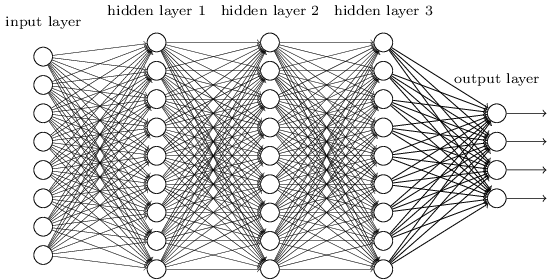
\includegraphics[width=\textwidth]{neuralnet.png}
\centering
\caption{A Neural Network with 1 input layer, 3 hidden layers and 1 output layer. This represents a densely connected neural network, where each node is connected to every node of the preceding and subsequent layers. At each node, linking functions can be had }
\end{figure}

Figure 1 depicts a sample neural network with 5 layers, with 8 data points as input, and 3 data points as output. In such a network, we would train it by providing the input data and output data, and letting the network learn how to integrate the inputs to create a network of activations that can be used to produce the corresponding output. This in part mimics the way we learn - experience teaches us that certain stimuli will result in specific effects (when we see a lightning bolt, we can expect the sound of thunder), and thus when new input comes in (a lightning bolt is seen), we can predict that the output that would arise (thunder is heard). In variant calling, deep learning will allow us to predict based on variant calling patterns and data whether a variant is valid and exists, or is erroneous. This will allow us to draw of the diversity of data with different variant callers, through letting the network learn which patterns will result in a valid call and which patterns are actually false positives. It will also allow us to tap on the differential sensitivity of different callers, as the neural network is able to learn which callers work best for which types of mutations. Thus, such a combinatorial approach will allow us to improve the accuracy and precision of variant calling.\\


\begin{equation}
P(Mutation is Important | Mutation is clinVar) = \frac{P(Mutation is clinVar | mutation is important)* P(Mutation is important)}{P(Mutation is ClinVar)}
\end{equation}


\begin{equation}
\prod P(token_i | spam) = P("free" | spam)* P("viagra"|spam)*P(next token|spam)....
\end{equation}

\begin{equation}
P(clinVar | important) 
\end{equation}
\begin{equation}
P(mutationTaster | important)
\end{equation}
\begin{equation}
P(SIFT | important)
\end{equation}

\section{Materials and Methods}

\subsection{Artificial Datasets}
To generate datasets to train variant calling networks, VarSim was used with ART in order to generate artificial datasets. Datasets generated has 


\subsection{Variant Callers}
Variant callers were chosen for our neural network based on their orthogonal calling and reference methodologies - we wanted to maximise the range of variant callers in order to optimise the information that the neural network receives (See Table N). We used two haplotype based callers, FreeBayes (Garrison \& Marth, 2012) and GATK Haplotype Caller (McKenna et al. 2010, DePristo et al. 2011), two position based callers GATK unified Genotyper and Samtools (Li H, et al., 2009) and finally Pindel, a pattern growth based caller (Ye et al., 2009). The features and differences of all 5 callers can be found in Table 1.  All callers have been well studied and are commonly used in variant calling pipelines (Sandmann et al., 2017, Hwang et al., 2015 Xie et al., 2014 and Liu et al., 2013). 

\begin{table}[h]
\caption{Table Comparing Methods and Features of Different variant callers.}
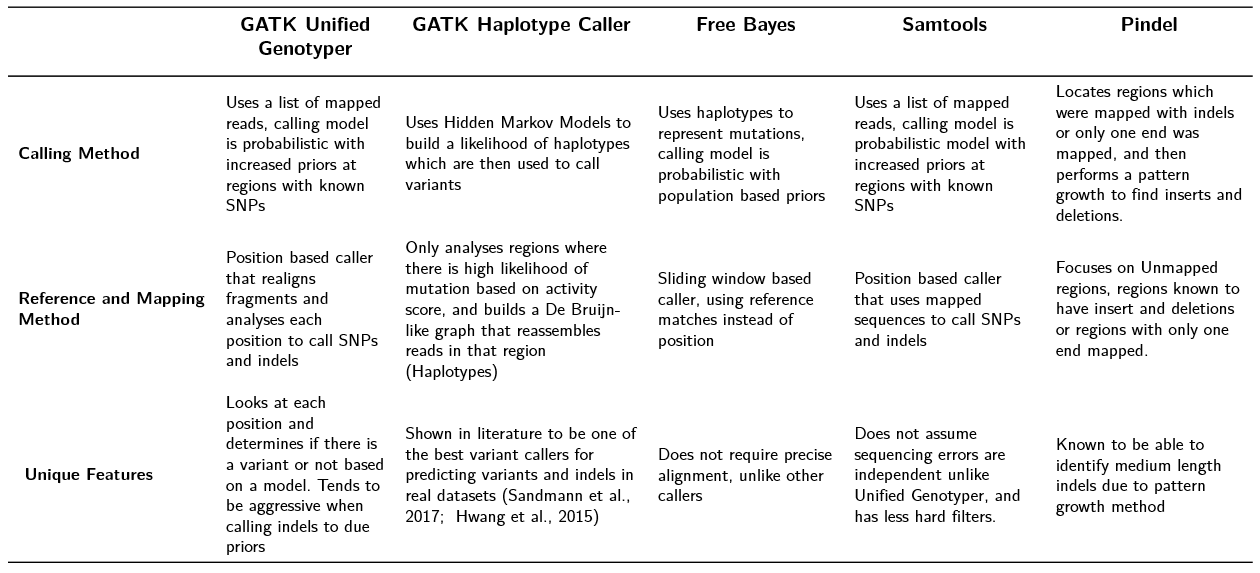
\includegraphics[width=\textwidth]{analysisofvariantcallers.png}
\centering
\end{table}

REFERENCES : \\
Samtools : Li H, et al., 2009\\
GATK UG/HC : McKenna et al. 2010, DePristo et al. 2011\\
FB : Garrison \& Marth, 2012\\
Pindel : Ye et al., 2009\\

\subsection{Feature Selection}

\subsection{Neural Networks}



\subsection{Technologies}
For our deep learning networks, we used the Keras library with a TensorFlow backend. TensorFlow was chosen due to its superior performance on single machines with multiple cores. On our Ubuntu compute cluster, TensorFlow's distributed CPU computation and queue management system enabled better performance in network training compared to other backend machine learning technologies technologies. For more explanation on the algorithms underpinning deep learning, see Appendix (INSERT) for more information 

The general programming platform used was Python. Python was chosen due to its access to various important libraries, including NumPy, SciPy, Pomegrenate and PyVCF. NumPy was used to prepare input vectors for deep learning training, SciPy was used to perform Principal Component Analysis and Synthetic Minority Oversampling Technique Methods (See Appedndix INSERT) for more information. Pomegranate was used to generate and compute the probabilistic model and ranking system for our Bayesian Network (INSERT see MM methods section N for more information). Finally, PyVCF was used to parse the VCF files into python objects for easy manipulation.

\subsection{Feature Engineering}
In order to train the neural network, features were extracted from the variant callers, as well as engineered from the original dataset. All the features used in the training can be found in table N. More information and descriptions of the mathematics behind the engineered features can be found in appendix INSERT.

\begin{table}[]
\caption{Feature Engineering Table}
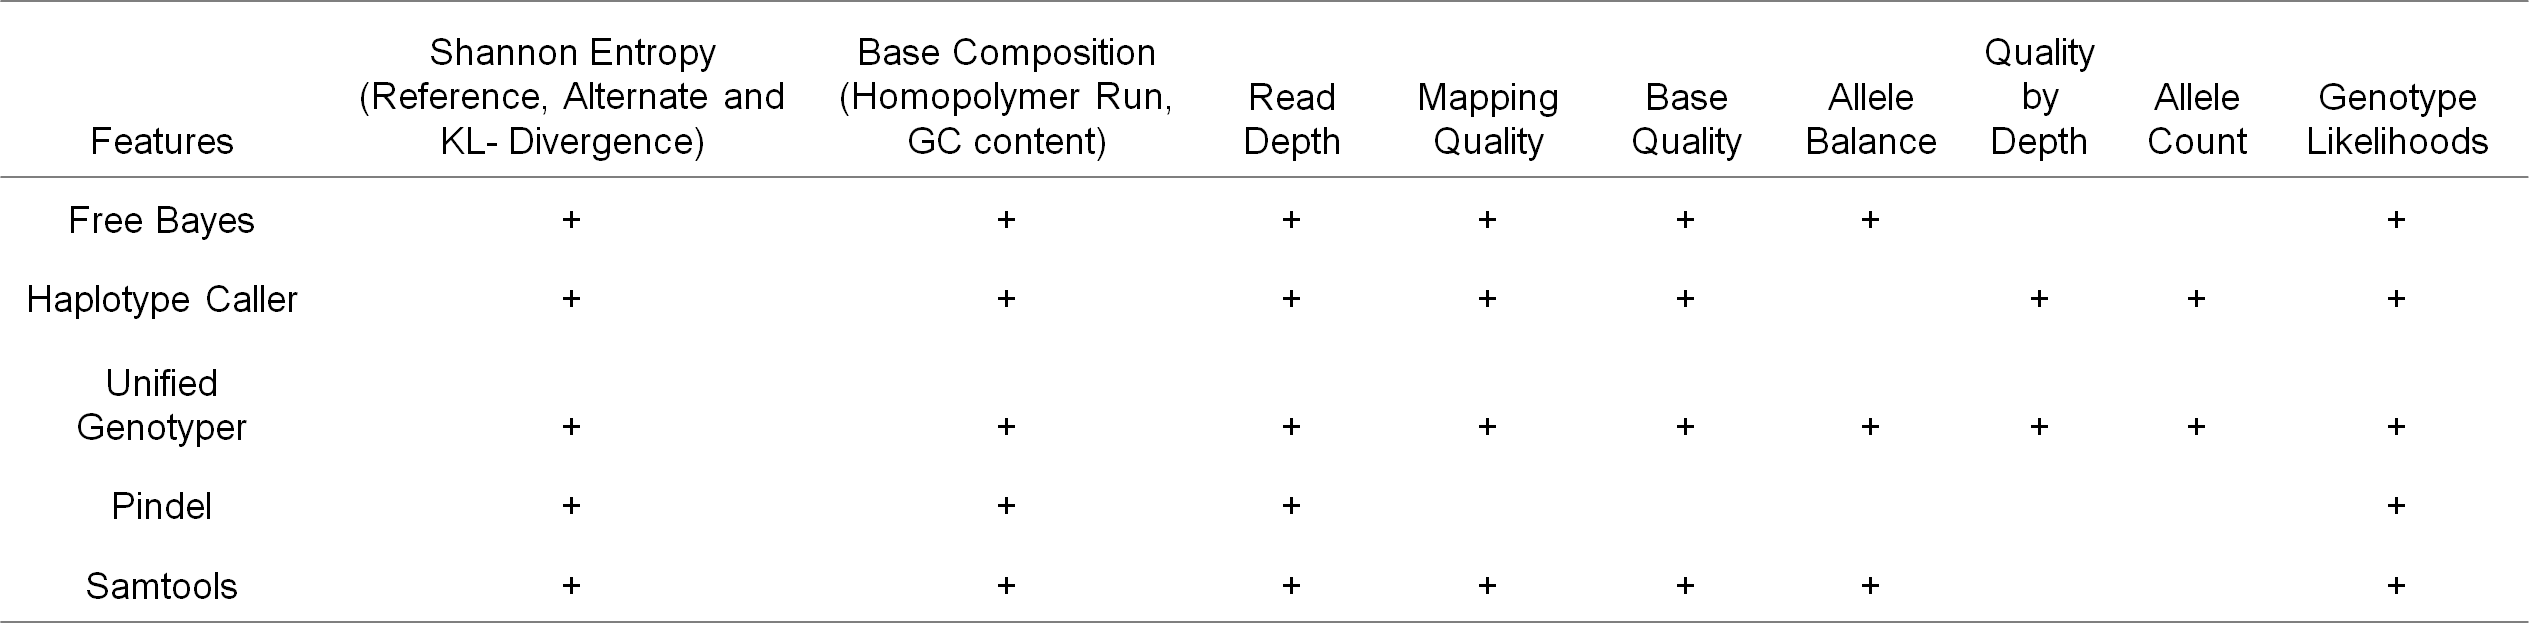
\includegraphics[width=\textwidth]{featureengineering.png}
\centering
\end{table}


\subsection{Artificial Datasets}

\subsection{Processing tools}

\subsection{PDX datasets}


\section{Results and Discussion}
\subsection{Generation of Artificial Genome}
In order to begin training 



\subsection{Network Architecture}
We systematically tested out various neural network architectures to see which architecture would perform the best. The architectures tested out were the flat architecture with 7 densely connected layers of 80 nodes each, the PCA + flat architecture which had the same neural network architecture, but before the input data was fed into the network a Principal Components Analysis was done to reduce the dataset to 8 principal components which was then used as input data for the neural network. Finally, the last architecture we tested was the merged network. The overall structure of the networks can be seen in Figure N. \\\\

\begin{figure}[H]
\caption{Feature Engineering Table}
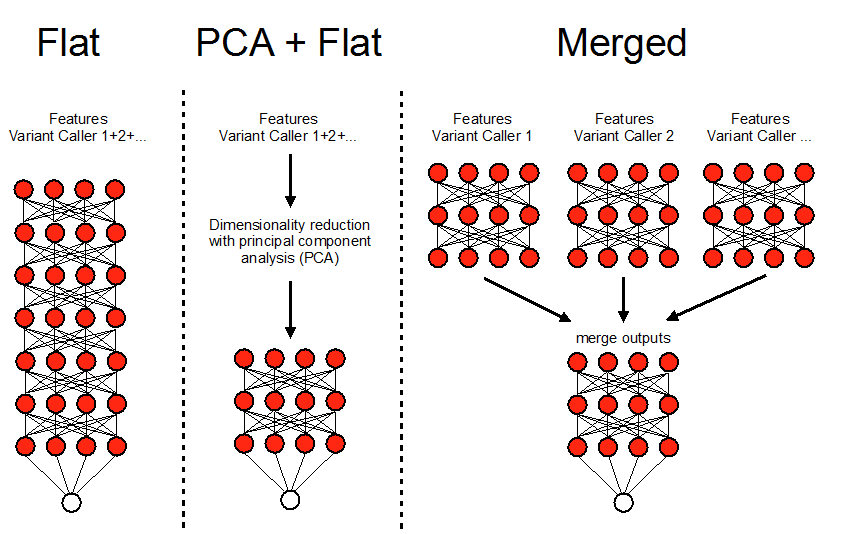
\includegraphics[width=\textwidth]{neuralnetworkstructure.png}
\centering
\end{figure}

\begin{figure}[H]
\caption{Feature Engineering Table}
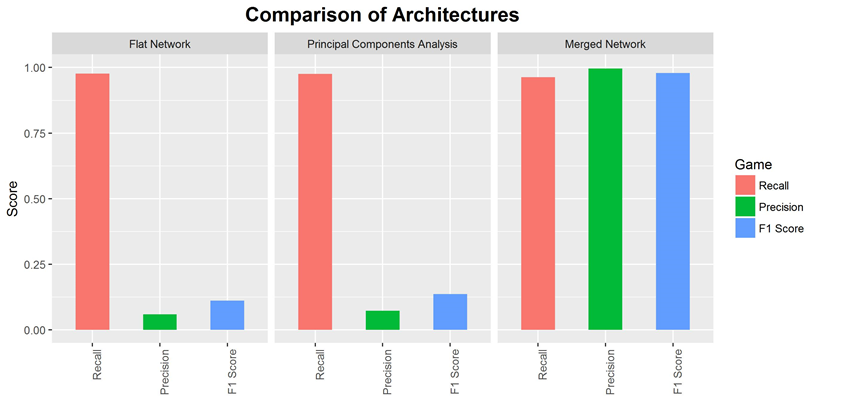
\includegraphics[width=\textwidth]{neuralnetworkstructureresults.png}
\centering
\end{figure}
Initially, with the flat network, the precision rate was very low, indicating that the neural network was unable to learn from the input feature set. We suspected that this was due to high dimensionality in the dataset, which led to our second architecture design, the PCA with flat analysis. Principal components analysis has been shown to be able to successfully improve learning in high dimensionality datasets (Chen et al., 2014; Van Der Maaten, Postma \& Van den Herik, 2009). Ultimately both failed to learn, indicating to us that perhaps the features from each of the callers had to be analysed separately before being passed into a separate neural network that did the final score computations. With this merged network, we managed to obtain a decent precision and F1 score that was far better than the previous two architectures. 


\subsection{Network Tuning and Optimisation}

A. Sample Balancing

In tuning our network, we sought to study how the various hyperparameters as well as the datastructure affected our network's ability to learn from the data. In particular, we focused on four issues, sample balancing, optimiser choise, learning rate choice and number of layers. These four issues are known to be critical in deep learning networks (CITATION x4). Our first concern was sample balancing - the simulated dataset contained an imbalance of positive training examples versus negative training examples. Such an sample imbalance has been known to affect learning adversely (Yan et al., 2015; López et al., 2012). Thus, we sought to study two methods of sample balancing, undersampling and oversampling. Our data was skewed with a high amount of negative training samples and  a low number of positive train samples. Thus, undersampling was implemented by removing negative training examples until the number of negative training examples was equal to the number of positive training examples. In oversampling, the Synthetic Minority Oversampling Technique(SMOTE) was done, which uses nearest neighbours to create more datapoints for the positive training example (see Appendix INSERT for more details). Figure 1 shows a representation of the normal, datasets on two principal components. Performance of all three methods 	


\begin{figure}[H]
\caption{Feature Engineering Table}
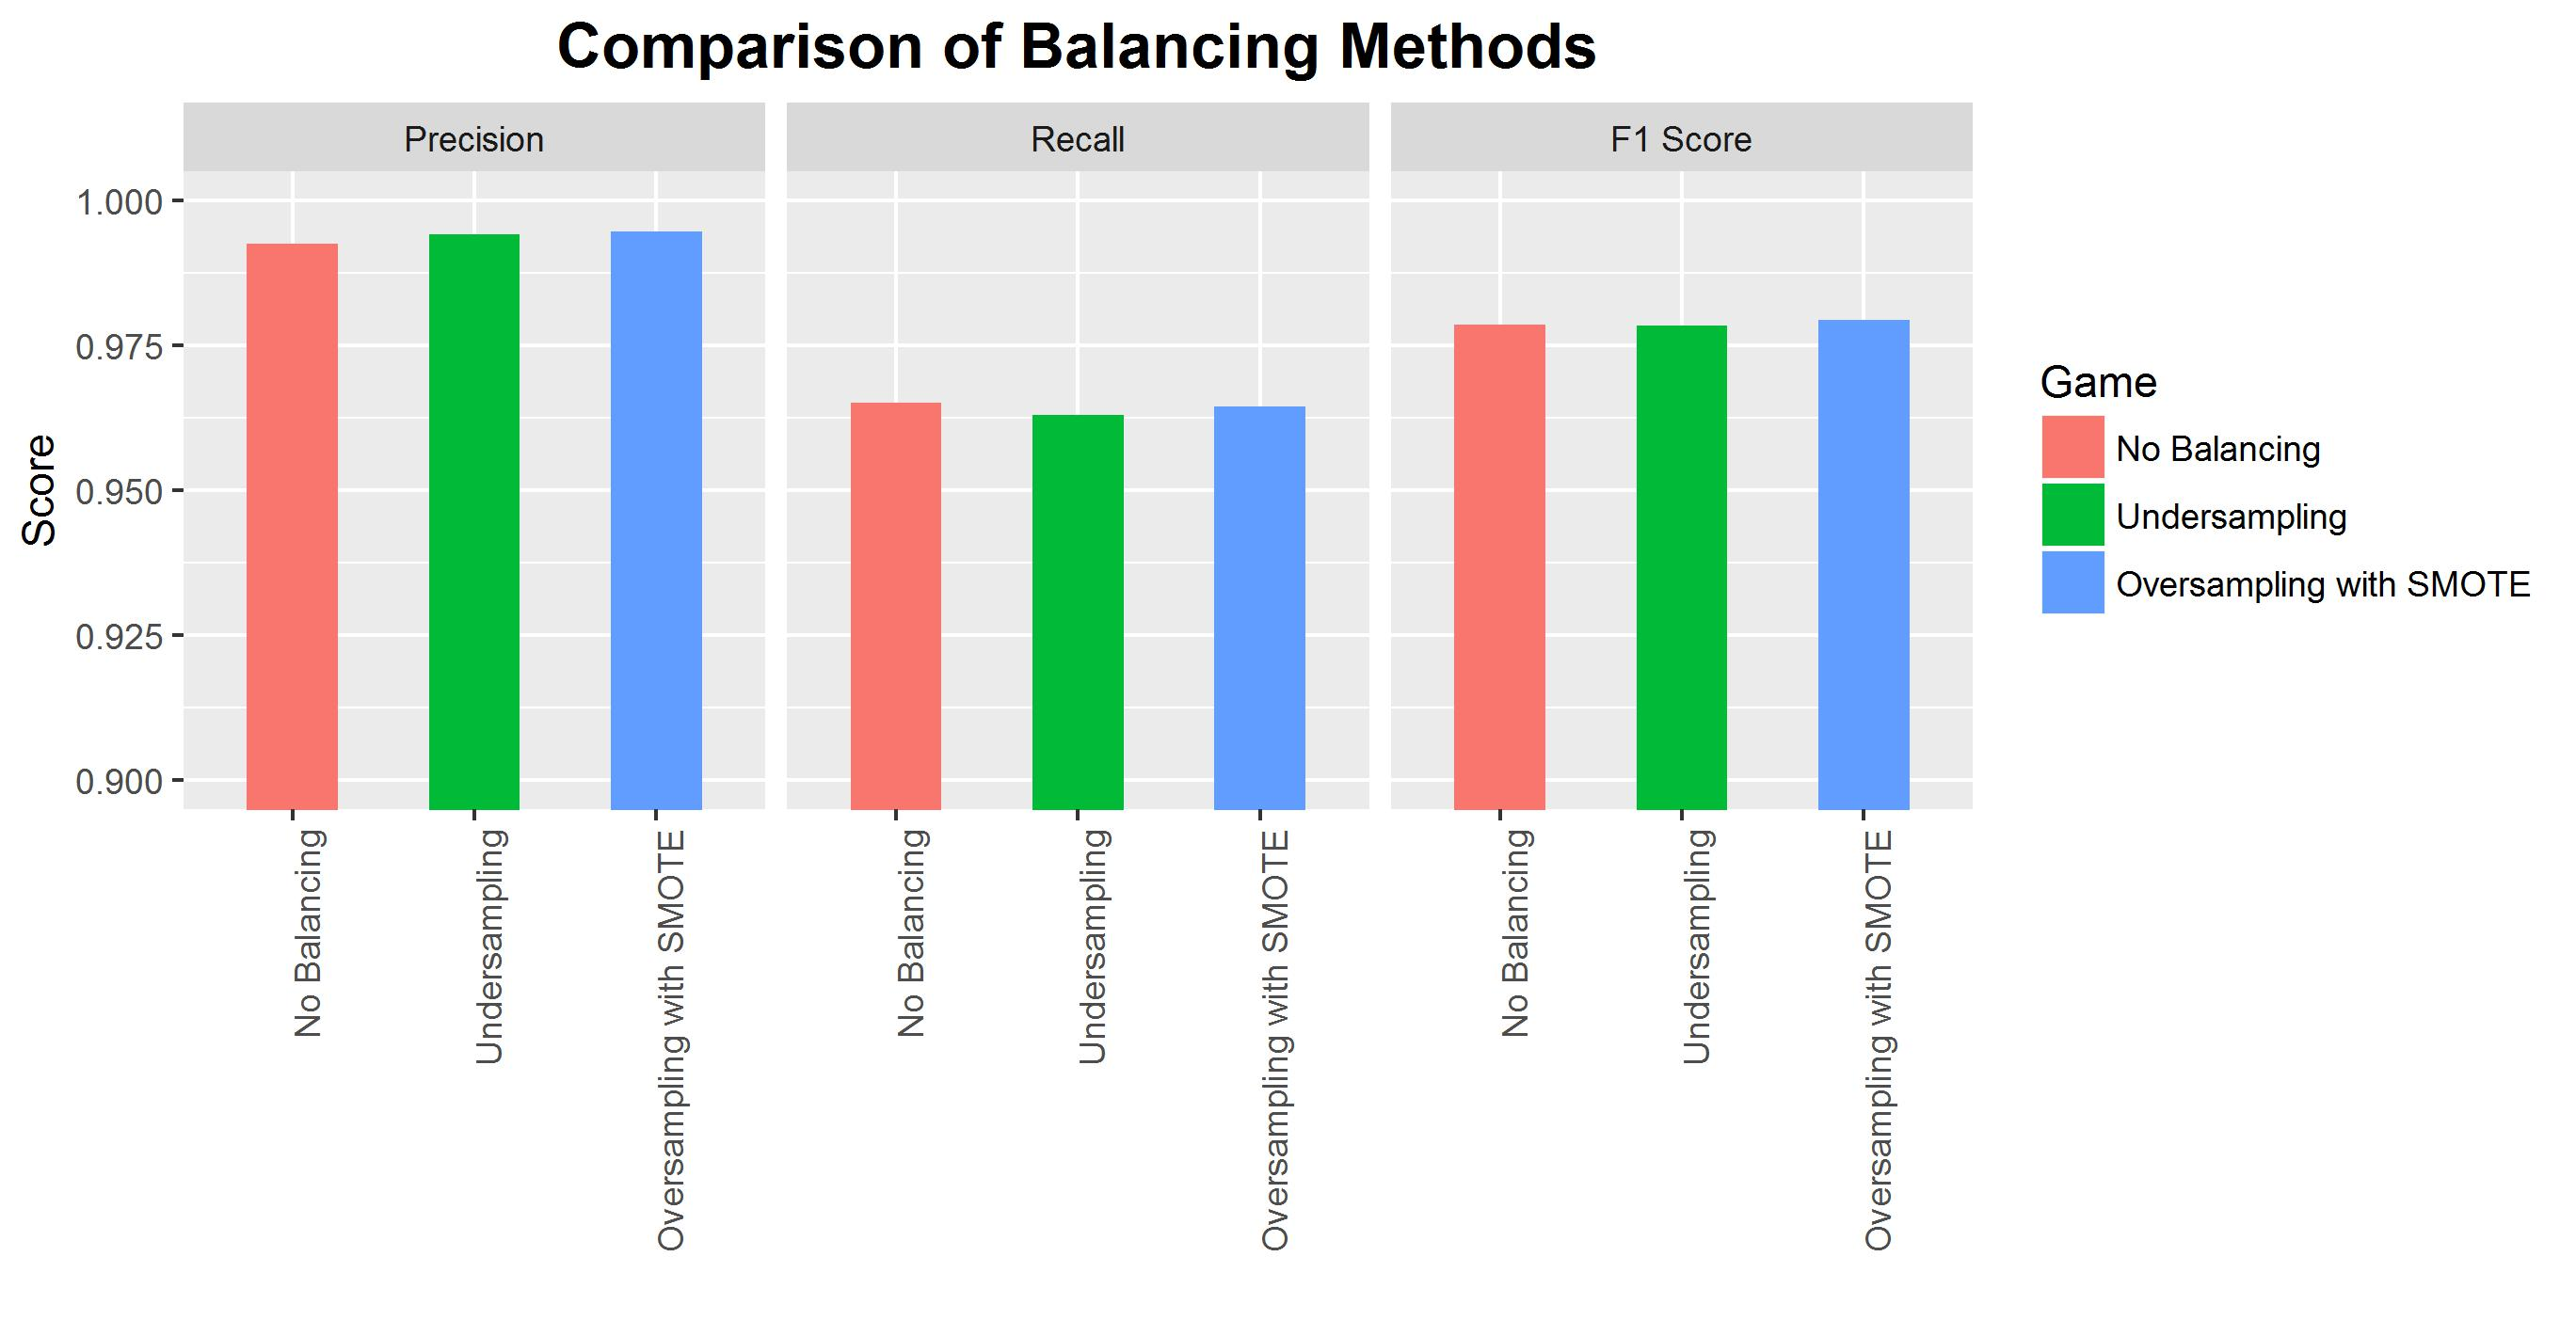
\includegraphics[width=\textwidth]{comparisonofbalancingmethods.png}
\centering
\end{figure}

B. Optimiser Choice
Optimisers have also been 

C. Learning Rate Choice



D. Number of Layers 



\subsection{Benchmarking of Network with Mason Datasets}
t

\subsection{Benchmarking of Network with NA Datasets}


\subsection{Analysis of PDX dataset using Bayesian Ranking systems}

\section{Future Directions}


\section{Appendixes}
\subsection{Key Technologies}


\section{Acknowledgements}

\section{Bibilography}

\begin{thebibliography}{9}
\bibitem{latexcompanion} 
O'Rawe, J., Jiang, T., Sun, G., Wu, Y., Wang, W., Hu, J., ... \& Wei, Z. (2013). Low concordance of multiple variant-calling pipelines: practical implications for exome and genome sequencing. Genome medicine, 5(3), 1.
 
\bibitem{einstein} 
 Cornish, A., \& Guda, C. (2015). A comparison of variant calling pipelines using genome in a bottle as a reference. BioMed research international, 2015.

\bibitem{knuthwebsite} 
Mohiyuddin, M., Mu, J. C., Li, J., Asadi, N. B., Gerstein, M. B., Abyzov, A., ... \& Lam, H. Y. (2015). MetaSV: an accurate and integrative structural-variant caller for next generation sequencing. Bioinformatics, btv204.

\bibitem{knuthwebsite} 
Gézsi, A., Bolgár, B., Marx, P., Sarkozy, P., Szalai, C., \& Antal, P. (2015). VariantMetaCaller: automated fusion of variant calling pipelines for quantitative, precision-based filtering. BMC genomics, 16(1), 1.

\bibitem{knuthwebsite} 
Huval, B., Wang, T., Tandon, S., Kiske, J., Song, W., Pazhayampallil, J., Andriluka, M., Rajpurkar, P., Migimatsu, T., Cheng-Yue, R. and Mujica, F., 2015. An empirical evaluation of deep learning on highway driving. arXiv preprint arXiv:1504.01716.

\end{thebibliography}



\end{document}